% vim: set spell spelllang=en tw=100 et sw=4 sts=4 foldmethod=marker foldmarker={{{,}}} :

\documentclass{beamer}

\usepackage{tikz}
\usepackage{xcolor}
\usepackage{complexity}
\usepackage{hyperref}
\usepackage{microtype}
\usepackage{amsmath}                   % \operatorname
\usepackage{amsfonts}                  % \mathcal
\usepackage{amssymb}                   % \nexists
\usepackage{gnuplot-lua-tikz}          % graphs
\usepackage[vlined]{algorithm2e} % algorithms
\usepackage{centernot}

\newcommand{\McSplit}{\textproc{McSplit}}

\usetikzlibrary{shapes, arrows, shadows, calc, positioning, fit}
\usetikzlibrary{decorations.pathreplacing, decorations.pathmorphing, shapes.misc}
\usetikzlibrary{tikzmark}

\definecolor{uofguniversityblue}{rgb}{0, 0.219608, 0.396078}

\definecolor{uofgheather}{rgb}{0.356863, 0.32549, 0.490196}
\definecolor{uofgaquamarine}{rgb}{0.603922, 0.72549, 0.678431}
\definecolor{uofgslate}{rgb}{0.309804, 0.34902, 0.380392}
\definecolor{uofgrose}{rgb}{0.823529, 0.470588, 0.709804}
\definecolor{uofgmocha}{rgb}{0.709804, 0.564706, 0.47451}
\definecolor{uofgsandstone}{rgb}{0.321569, 0.278431, 0.231373}
\definecolor{uofgforest}{rgb}{0, 0.2, 0.129412}
\definecolor{uofglawn}{rgb}{0.517647, 0.741176, 0}
\definecolor{uofgcobalt}{rgb}{0, 0.615686, 0.92549}
\definecolor{uofgturquoise}{rgb}{0, 0.709804, 0.819608}
\definecolor{uofgsunshine}{rgb}{1.0, 0.862745, 0.211765}
\definecolor{uofgpumpkin}{rgb}{1.0, 0.72549, 0.282353}
\definecolor{uofgthistle}{rgb}{0.584314, 0.070588, 0.447059}
\definecolor{uofgrust}{rgb}{0.603922, 0.227451, 0.023529}
\definecolor{uofgburgundy}{rgb}{0.490196, 0.133333, 0.223529}
\definecolor{uofgpillarbox}{rgb}{0.701961, 0.047059, 0}
\definecolor{uofglavendar}{rgb}{0.356863, 0.301961, 0.580392}

\tikzset{vertex/.style={draw, circle, inner sep=0pt, minimum size=0.5cm, font=\small\bfseries}}
\tikzset{notvertex/.style={vertex, color=white, text=black}}
\tikzset{plainvertex/.style={vertex}}
\tikzset{vertexc1/.style={vertex, fill=uofgburgundy, text=white}}
\tikzset{vertexc2/.style={vertex, fill=uofgsandstone, text=white}}
\tikzset{vertexc3/.style={vertex, fill=uofgforest, text=white}}
\tikzset{vertexc4/.style={vertex, fill=uofgheather, text=white}}
\tikzset{edge/.style={color=black, ultra thick}}
\tikzset{lledge/.style={color=uofgsandstone!50!white, thin}}
\tikzset{ledge/.style={color=uofgsandstone!50!white, thick}}
\tikzset{bedge/.style={ultra thick}}

% {{{ theme things
\useoutertheme[footline=authortitle]{miniframes}
\useinnertheme{rectangles}

\setbeamerfont{block title}{size={}}
\setbeamerfont{title}{size=\large,series=\bfseries}
\setbeamerfont{section title}{size=\large,series=\mdseries}
\setbeamerfont{author}{size=\normalsize,series=\mdseries}
\setbeamercolor*{structure}{fg=uofguniversityblue}
\setbeamercolor*{palette primary}{use=structure,fg=black,bg=white}
\setbeamercolor*{palette secondary}{use=structure,fg=white,bg=uofgcobalt}
\setbeamercolor*{palette tertiary}{use=structure,fg=white,bg=uofguniversityblue}
\setbeamercolor*{palette quaternary}{fg=white,bg=black}

\setbeamercolor*{titlelike}{parent=palette primary}

\beamertemplatenavigationsymbolsempty

\usetikzlibrary{graphs}

\newcommand{\exampleG} {
  \tikz {
    \visible<-2> {
        \graph [nodes={draw, circle, minimum width=.4cm, inner sep=1pt}, circular placement, radius=0.6cm,
                clockwise=4, phase=45] {
                  1[fill=white],2[fill=white],3[fill=white],4[fill=white];
            1--4; 2--3; 2--4; 3--4;
        };
    }
    \visible<3> {
        \graph [nodes={draw, circle, minimum width=.4cm, inner sep=1pt}, circular placement, radius=0.6cm,
                clockwise=4, phase=45] {
                  1[fill=uofgpumpkin],2[fill=white],3[fill=uofgpumpkin],4[fill=uofgpumpkin];
            1--4; 2--3; 2--4; 3--4;
        };
    }
  }
}
\newcommand{\exampleH} {
  \tikz {
    \visible<-2> {
        \graph [nodes={draw, circle, minimum width=.4cm, inner sep=1pt}, circular placement, radius=0.6cm,
                clockwise=4, phase=45] {
                  a[fill=white],b[fill=white],c[fill=white],d[fill=white];
            a--b; b--c; c--d; d--a;
        };
    }
    \visible<3> {
        \graph [nodes={draw, circle, minimum width=.4cm, inner sep=1pt}, circular placement, radius=0.6cm,
                clockwise=4, phase=45] {
                  a[fill=uofgpumpkin],b[fill=white],c[fill=uofgpumpkin],d[fill=uofgpumpkin];
            a--b; b--c; c--d; d--a;
        };
    }
  }
}

\setbeamertemplate{title page}
{
    \begin{tikzpicture}[remember picture, overlay]
        \node at (current page.north west) {
            \begin{tikzpicture}[remember picture, overlay]
                \fill [fill=uofguniversityblue, anchor=north west] (0, 0) rectangle (\paperwidth, -2.6cm);
            \end{tikzpicture}
        };

        \node (logo) [anchor=north east, shift={(-0.3cm,-0.6cm)}] at (current page.north east) {
            \includegraphics*[keepaspectratio=true,scale=0.65]{UoG_keyline.pdf}
        };

        \node [anchor=west, xshift=0.2cm] at (current page.west |- logo.west) {
            \begin{minipage}{0.65\paperwidth}\raggedright
                {\usebeamerfont{title}\usebeamercolor[white]{}\inserttitle}\\[0.1cm]
                {\usebeamerfont{author}\usebeamercolor[white]{}\insertauthor}
            \end{minipage}
        };
    \end{tikzpicture}
}

\setbeamertemplate{section page}
{
    \begin{centering}
        \begin{beamercolorbox}[sep=12pt,center]{part title}
            \usebeamerfont{section title}\insertsection\par
        \end{beamercolorbox}
    \end{centering}
}

\newcommand{\frameofframes}{/}
\newcommand{\setframeofframes}[1]{\renewcommand{\frameofframes}{#1}}

\makeatletter
\setbeamertemplate{footline}
{%
    \begin{beamercolorbox}[colsep=1.5pt]{upper separation line foot}
    \end{beamercolorbox}
    \begin{beamercolorbox}[ht=2.5ex,dp=1.125ex,%
        leftskip=.3cm,rightskip=.3cm plus1fil]{author in head/foot}%
        \leavevmode{\usebeamerfont{author in head/foot}\insertshortauthor}%
        \hfill%
        {\usebeamerfont{institute in head/foot}\usebeamercolor[fg]{institute in head/foot}\insertshortinstitute}%
    \end{beamercolorbox}%
    \begin{beamercolorbox}[ht=2.5ex,dp=1.125ex,%
        leftskip=.3cm,rightskip=.3cm plus1fil]{title in head/foot}%
        {\usebeamerfont{title in head/foot}\insertshorttitle}%
        \hfill%
        {\usebeamerfont{frame number}\usebeamercolor[fg]{frame number}\insertframenumber~\frameofframes~\inserttotalframenumber}
    \end{beamercolorbox}%
    \begin{beamercolorbox}[colsep=1.5pt]{lower separation line foot}
    \end{beamercolorbox}
}

\makeatletter
\newenvironment{nearlyplainframe}[2][]{
    \def\beamer@entrycode{\vspace*{-\headheight}\vspace*{3pt}}
    \setbeamertemplate{headline}
    {%
        \begin{beamercolorbox}[colsep=1.5pt]{upper separation line head}
        \end{beamercolorbox}
        \begin{beamercolorbox}[ht=0.5ex,dp=0.125ex,%
            leftskip=.3cm,rightskip=.3cm plus1fil]{title in head/foot}%
        \end{beamercolorbox}%
        \begin{beamercolorbox}[ht=0.5ex,dp=0.125ex,%
            leftskip=.3cm,rightskip=.3cm plus1fil]{author in head/foot}%
        \end{beamercolorbox}%
        \begin{beamercolorbox}[colsep=1.5pt]{lower separation line head}
        \end{beamercolorbox}
        \vspace*{\headheight}
    }

    \setbeamertemplate{footline}
    {%
        \begin{beamercolorbox}[colsep=1.5pt]{upper separation line foot}
        \end{beamercolorbox}
        \begin{beamercolorbox}[ht=0.5ex,dp=0.125ex,%
            leftskip=.3cm,rightskip=.3cm plus1fil]{author in head/foot}%
        \end{beamercolorbox}%
        \begin{beamercolorbox}[ht=0.5ex,dp=0.125ex,%
            leftskip=.3cm,rightskip=.3cm plus1fil]{title in head/foot}%
        \end{beamercolorbox}%
        \begin{beamercolorbox}[colsep=1.5pt]{lower separation line foot}
        \end{beamercolorbox}
    }

    \begin{frame}[#1]{#2}
    }{
    \end{frame}
}
\makeatother

% }}}

\title[A Partitioning Algorithm for Maximum Common Subgraph Problems]{A Partitioning Algorithm for \\
Maximum Common Subgraph Problems}
\author[Ciaran McCreesh, Patrick Prosser and James Trimble]{Ciaran McCreesh, Patrick
Prosser, and \\ James Trimble}

\begin{document}

{
    \usebackgroundtemplate{
        \tikz[overlay, remember picture]
        \node[at=(current page.south), anchor=south, inner sep=0pt]{\includegraphics*[keepaspectratio=true, width=\paperwidth]{background.jpg}};
    }
    \begin{frame}[plain,noframenumbering]
        \titlepage
    \end{frame}
}

\begin{frame}{Maximum Common Subgraph Problems}
\begin{columns}[T]
  \begin{column}{0.47\textwidth}
    \centering
    \textbf{Induced}

    \begin{center}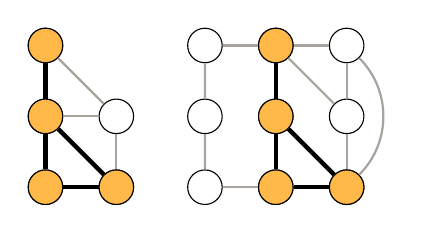
\begin{tikzpicture}[scale=0.45]
        \visible<1> {
          \node[draw, circle, fill=white, inner sep=2.5pt, font=\bfseries] (Na) at (1,  0) {\vphantom{0}};
          \node[draw, circle, fill=white, inner sep=2.5pt, font=\bfseries] (Nb) at (1, -2) {\vphantom{0}};
          \node[draw, circle, fill=white, inner sep=2.5pt, font=\bfseries] (Nc) at (1, -4) {\vphantom{0}};
          \node[draw, circle, fill=white, inner sep=2.5pt, font=\bfseries] (Nd) at (3, -4) {\vphantom{0}};
        }
        \visible<2-> {
          \node[draw, circle, fill=uofgpumpkin, inner sep=2.5pt, font=\bfseries] (Na) at (1,  0) {\vphantom{0}};
          \node[draw, circle, fill=uofgpumpkin, inner sep=2.5pt, font=\bfseries] (Nb) at (1, -2) {\vphantom{0}};
          \node[draw, circle, fill=uofgpumpkin, inner sep=2.5pt, font=\bfseries] (Nc) at (1, -4) {\vphantom{0}};
          \node[draw, circle, fill=uofgpumpkin, inner sep=2.5pt, font=\bfseries] (Nd) at (3, -4) {\vphantom{0}};
        }
        \node[draw, circle, fill=white, inner sep=2.5pt, font=\bfseries] (Ne) at (3, -2) {\vphantom{0}};

        \visible<1> {
          \draw [ledge] (Na) -- (Nb);
          \draw [ledge] (Nb) -- (Nc);
          \draw [ledge] (Nc) -- (Nd);
          \draw [ledge] (Nb) -- (Nd);
        }
        \visible<2-> {
          \draw [edge] (Na) -- (Nb);
          \draw [edge] (Nb) -- (Nc);
          \draw [edge] (Nc) -- (Nd);
          \draw [edge] (Nb) -- (Nd);
        }
        \draw [ledge] (Na) -- (Ne);
        \draw [ledge] (Nb) -- (Ne);
        \draw [ledge] (Nd) -- (Ne);

        \visible<1> {
          \node[draw, circle, fill=white, inner sep=2.5pt, font=\bfseries] (N1) at (7.5,  0) {\vphantom{0}};
          \node[draw, circle, fill=white, inner sep=2.5pt, font=\bfseries] (N3) at (7.5, -2) {\vphantom{0}};
          \node[draw, circle, fill=white, inner sep=2.5pt, font=\bfseries] (N5) at (7.5, -4) {\vphantom{0}};
          \node[draw, circle, fill=white, inner sep=2.5pt, font=\bfseries] (N6) at (9.5, -4) {\vphantom{0}};
        }
        \visible<2-> {
          \node[draw, circle, fill=uofgpumpkin, inner sep=2.5pt, font=\bfseries] (N1) at (7.5,  0) {\vphantom{0}};
          \node[draw, circle, fill=uofgpumpkin, inner sep=2.5pt, font=\bfseries] (N3) at (7.5, -2) {\vphantom{0}};
          \node[draw, circle, fill=uofgpumpkin, inner sep=2.5pt, font=\bfseries] (N5) at (7.5, -4) {\vphantom{0}};
          \node[draw, circle, fill=uofgpumpkin, inner sep=2.5pt, font=\bfseries] (N6) at (9.5, -4) {\vphantom{0}};
        }
        \node[draw, circle, fill=white, inner sep=2.5pt, font=\bfseries] (N2) at (9.5,  0) {\vphantom{0}};
        \node[draw, circle, fill=white, inner sep=2.5pt, font=\bfseries] (N4) at (9.5, -2) {\vphantom{0}};
        \node[draw, circle, fill=white, inner sep=2.5pt, font=\bfseries] (N7) at (5.5,  0) {\vphantom{0}};
        \node[draw, circle, fill=white, inner sep=2.5pt, font=\bfseries] (N8) at (5.5, -2) {\vphantom{0}};
        \node[draw, circle, fill=white, inner sep=2.5pt, font=\bfseries] (N9) at (5.5, -4) {\vphantom{0}};

        \visible<1> {
          \draw [ledge] (N1) -- (N3);
          \draw [ledge] (N3) -- (N5);
          \draw [ledge] (N3) -- (N6);
          \draw [ledge] (N5) -- (N6);
        }
        \visible<2-> {
          \draw [edge] (N1) -- (N3);
          \draw [edge] (N3) -- (N5);
          \draw [edge] (N3) -- (N6);
          \draw [edge] (N5) -- (N6);
        }
        \draw [ledge] (N1) -- (N2);
        \draw [ledge] (N1) -- (N4);
        \draw [ledge] (N1) -- (N7);
        \draw [ledge] (N2) -- (N4);
        \draw [ledge] (N2) to [in=45, out=315] (N6);
        \draw [ledge] (N4) -- (N6);
        \draw [ledge] (N5) -- (N9);
        \draw [ledge] (N7) -- (N8);
        \draw [ledge] (N8) -- (N9);
    \end{tikzpicture}\end{center}
  \end{column}

  \visible<3-> {
    \textcolor{gray}{\vrule{}}
  }

  \hspace{10pt}

  \begin{column}{0.47\textwidth}
    \visible<3-> {
      \centering
      \textbf{Partial}

      \begin{center}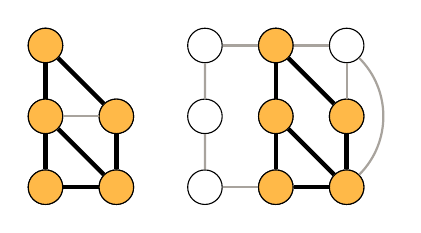
\begin{tikzpicture}[scale=0.45]
        \visible<3> {
          \node[draw, circle, fill=white, inner sep=2.5pt, font=\bfseries] (Na) at (1,  0) {\vphantom{0}};
          \node[draw, circle, fill=white, inner sep=2.5pt, font=\bfseries] (Nb) at (1, -2) {\vphantom{0}};
          \node[draw, circle, fill=white, inner sep=2.5pt, font=\bfseries] (Nc) at (1, -4) {\vphantom{0}};
          \node[draw, circle, fill=white, inner sep=2.5pt, font=\bfseries] (Nd) at (3, -4) {\vphantom{0}};
          \node[draw, circle, fill=white, inner sep=2.5pt, font=\bfseries] (Ne) at (3, -2) {\vphantom{0}};
        }
        \visible<4-> {
          \node[draw, circle, fill=uofgpumpkin, inner sep=2.5pt, font=\bfseries] (Na) at (1,  0) {\vphantom{0}};
          \node[draw, circle, fill=uofgpumpkin, inner sep=2.5pt, font=\bfseries] (Nb) at (1, -2) {\vphantom{0}};
          \node[draw, circle, fill=uofgpumpkin, inner sep=2.5pt, font=\bfseries] (Nc) at (1, -4) {\vphantom{0}};
          \node[draw, circle, fill=uofgpumpkin, inner sep=2.5pt, font=\bfseries] (Nd) at (3, -4) {\vphantom{0}};
          \node[draw, circle, fill=uofgpumpkin, inner sep=2.5pt, font=\bfseries] (Ne) at (3, -2) {\vphantom{0}};
        }

        \visible<3> {
          \draw [ledge] (Na) -- (Nb);
          \draw [ledge] (Na) -- (Ne);
          \draw [ledge] (Nb) -- (Nc);
          \draw [ledge] (Nb) -- (Nd);
          \draw [ledge] (Nc) -- (Nd);
          \draw [ledge] (Nd) -- (Ne);
          \draw [ledge] (Nb) -- (Ne);
        }
        \visible<4-> {
          \draw [edge] (Na) -- (Nb);
          \draw [edge] (Na) -- (Ne);
          \draw [edge] (Nb) -- (Nc);
          \draw [edge] (Nb) -- (Nd);
          \draw [edge] (Nc) -- (Nd);
          \draw [edge] (Nd) -- (Ne);
          \draw [ledge] (Nb) -- (Ne);
        }

        \visible<3> {
          \node[draw, circle, fill=white, inner sep=2.5pt, font=\bfseries] (N1) at (7.5,  0) {\vphantom{0}};
          \node[draw, circle, fill=white, inner sep=2.5pt, font=\bfseries] (N3) at (7.5, -2) {\vphantom{0}};
          \node[draw, circle, fill=white, inner sep=2.5pt, font=\bfseries] (N4) at (9.5, -2) {\vphantom{0}};
          \node[draw, circle, fill=white, inner sep=2.5pt, font=\bfseries] (N5) at (7.5, -4) {\vphantom{0}};
          \node[draw, circle, fill=white, inner sep=2.5pt, font=\bfseries] (N6) at (9.5, -4) {\vphantom{0}};
        }
        \visible<4-> {
          \node[draw, circle, fill=uofgpumpkin, inner sep=2.5pt, font=\bfseries] (N1) at (7.5,  0) {\vphantom{0}};
          \node[draw, circle, fill=uofgpumpkin, inner sep=2.5pt, font=\bfseries] (N3) at (7.5, -2) {\vphantom{0}};
          \node[draw, circle, fill=uofgpumpkin, inner sep=2.5pt, font=\bfseries] (N4) at (9.5, -2) {\vphantom{0}};
          \node[draw, circle, fill=uofgpumpkin, inner sep=2.5pt, font=\bfseries] (N5) at (7.5, -4) {\vphantom{0}};
          \node[draw, circle, fill=uofgpumpkin, inner sep=2.5pt, font=\bfseries] (N6) at (9.5, -4) {\vphantom{0}};
        }
        \node[draw, circle, fill=white, inner sep=2.5pt, font=\bfseries] (N2) at (9.5,  0) {\vphantom{0}};
        \node[draw, circle, fill=white, inner sep=2.5pt, font=\bfseries] (N7) at (5.5,  0) {\vphantom{0}};
        \node[draw, circle, fill=white, inner sep=2.5pt, font=\bfseries] (N8) at (5.5, -2) {\vphantom{0}};
        \node[draw, circle, fill=white, inner sep=2.5pt, font=\bfseries] (N9) at (5.5, -4) {\vphantom{0}};

        \visible<3> {
          \draw [ledge] (N1) -- (N3);
          \draw [ledge] (N1) -- (N4);
          \draw [ledge] (N3) -- (N5);
          \draw [ledge] (N3) -- (N6);
          \draw [ledge] (N4) -- (N6);
          \draw [ledge] (N5) -- (N6);
        }
        \visible<4-> {
          \draw [edge] (N1) -- (N3);
          \draw [edge] (N1) -- (N4);
          \draw [edge] (N3) -- (N5);
          \draw [edge] (N3) -- (N6);
          \draw [edge] (N4) -- (N6);
          \draw [edge] (N5) -- (N6);
        }
        \draw [ledge] (N1) -- (N2);
        \draw [ledge] (N1) -- (N7);
        \draw [ledge] (N2) -- (N4);
        \draw [ledge] (N2) to [in=45, out=315] (N6);
        \draw [ledge] (N5) -- (N9);
        \draw [ledge] (N7) -- (N8);
        \draw [ledge] (N8) -- (N9);
      \end{tikzpicture}\end{center}
    }
  \end{column}
\end{columns}
\vspace{1cm}
\begin{itemize}
  \visible<5->{\item Each of these has a connected version}
  \visible<5->{\item Directed, undirected variants}
  \visible<5->{\item Edge and vertex labels}
  \visible<5->{\item I'll mainly talk about induced, unlabelled, unconnected,
      not-necessarily-connected}
\end{itemize}
\end{frame}

\begin{frame}{An Application in Chemistry}
  \centering
  \includegraphics*[keepaspectratio=true,width=0.6\textwidth]{raymond-willett-screenshot}
  \begin{itemize}
    \item Max Common Subgraph algorithms can be used to determine the degree of
      similarity between two molecules
    \item Image from (Raymond and Willett, 2002)
  \end{itemize}
\end{frame}

\begin{frame}{A Few Impractical Uses for a MCS Solvers}
    \begin{itemize}
        \item To find a maximum clique in graph $G$ with $n$ vertices,
          run MCIS($K_n$, $G$)
    \end{itemize}
    \begin{center}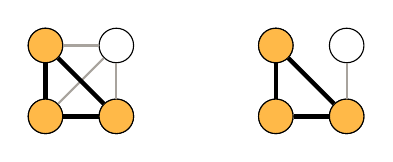
\begin{tikzpicture}[scale=0.45]
        \visible<2-> {
          \visible<-2> {
            \node[draw, circle, fill=white, inner sep=2.5pt, font=\bfseries] (Nb) at (1, -2) {\vphantom{0}};
            \node[draw, circle, fill=white, inner sep=2.5pt, font=\bfseries] (Nc) at (1, -4) {\vphantom{0}};
            \node[draw, circle, fill=white, inner sep=2.5pt, font=\bfseries] (Nd) at (3, -4) {\vphantom{0}};
          }
          \visible<3-> {
            \node[draw, circle, fill=uofgpumpkin, inner sep=2.5pt, font=\bfseries] (Nb) at (1, -2) {\vphantom{0}};
            \node[draw, circle, fill=uofgpumpkin, inner sep=2.5pt, font=\bfseries] (Nc) at (1, -4) {\vphantom{0}};
            \node[draw, circle, fill=uofgpumpkin, inner sep=2.5pt, font=\bfseries] (Nd) at (3, -4) {\vphantom{0}};
          }
          \node[draw, circle, fill=white, inner sep=2.5pt, font=\bfseries] (Ne) at (3, -2) {\vphantom{0}};

          \draw [ledge] (Nb) -- (Ne);
          \draw [ledge] (Nc) -- (Ne);
          \draw [ledge] (Nd) -- (Ne);
          \visible<-2> {
            \draw [ledge] (Nb) -- (Nc);
            \draw [ledge] (Nc) -- (Nd);
            \draw [ledge] (Nb) -- (Nd);
          }
          \visible<3-> {
            \draw [edge] (Nb) -- (Nc);
            \draw [edge] (Nc) -- (Nd);
            \draw [edge] (Nb) -- (Nd);
          }
        }

        \visible<-2> {
          \node[draw, circle, fill=white, inner sep=2.5pt, font=\bfseries] (N3) at (7.5, -2) {\vphantom{0}};
          \node[draw, circle, fill=white, inner sep=2.5pt, font=\bfseries] (N5) at (7.5, -4) {\vphantom{0}};
          \node[draw, circle, fill=white, inner sep=2.5pt, font=\bfseries] (N6) at (9.5, -4) {\vphantom{0}};
        }
        \visible<3-> {
          \node[draw, circle, fill=uofgpumpkin, inner sep=2.5pt, font=\bfseries] (N3) at (7.5, -2) {\vphantom{0}};
          \node[draw, circle, fill=uofgpumpkin, inner sep=2.5pt, font=\bfseries] (N5) at (7.5, -4) {\vphantom{0}};
          \node[draw, circle, fill=uofgpumpkin, inner sep=2.5pt, font=\bfseries] (N6) at (9.5, -4) {\vphantom{0}};
        }
        \node[draw, circle, fill=white, inner sep=2.5pt, font=\bfseries] (N4) at (9.5, -2) {\vphantom{0}};

        \visible<-2> {
          \draw [ledge] (N3) -- (N5);
          \draw [ledge] (N3) -- (N6);
          \draw [ledge] (N5) -- (N6);
        }
        \visible<3-> {
          \draw [edge] (N3) -- (N5);
          \draw [edge] (N3) -- (N6);
          \draw [edge] (N5) -- (N6);
        }
        \draw [ledge] (N4) -- (N6);
    \end{tikzpicture}\end{center}
    \begin{itemize}
      \visible<4-> {
        \item To test for a Hamiltonian cycle in graph $G$ with $n$ vertices,
            run MCPS($C_n$, $G$) and check if the result has $n$ edges.
      }
      \visible<5-> {
        \item Induced subgraph isomorphism: run MCIS, check if all vertices in the smaller graph are used
      }
      \visible<6-> {
        \item Non-induced subgraph isomorphism: run MCPS, check if all edges in the smaller graph are used
      }
    \end{itemize}
\end{frame}

\begin{frame}{Previous Algorithms}
    \begin{itemize}
        \item \textbf{Clique encoding} --- good for labelled instances
        \item \textbf{Constraint programming} --- good for unlabelled instances
            \begin{itemize}
                \item Using a dedicated implementation, not a CP toolkit
            \end{itemize}
        \item $\mathbf{k{\downarrow}}$ --- good for big instances
    \end{itemize}
\end{frame}

\begin{frame}{Clique Encoding}
  \begin{figure}[]
  \centering
      \exampleG
      \qquad
      \exampleH
  \end{figure}

  \include{scripts/clique_encoding}
\end{frame}

\begin{frame}{CP Model}
    \begin{itemize}
        \item A variable for each vertex in the pattern graph
        \item A value for each vertex in the target graph, and $\bot$
        \item Soft all-different constraint
        \item Maximise the number of non-$\bot$ values
    \end{itemize}
\end{frame}

\begin{frame}{The Observation Behind Our Algorithm}

    \begin{itemize}
        \item During search any two domains are identical or
            disjoint (with the exception of $\bot$)
    \end{itemize}

\end{frame}

\begin{frame}{The McSplit Algorithm}
    \begin{itemize}
        \item We can use a compact backtrackable data structure which splits vertices into
            partitions
        \item Propagation is just refining partitions
        \item Soft all-different can be calculated by counting rather than matching
    \end{itemize}
\end{frame}

\begin{frame}{Up or Down?}
    \begin{itemize}
        \item In our branch and bound algorithm, we try to find larger and larger common subgraphs
        \item We can go in the opposite direction (``McSplit-down'')
          \begin{itemize}
            \item first look for a common subgraph that uses all vertices in the smaller graph
            \item if that fails, look for a common subgraph that uses all but one of the vertices
            \item \dots and so on
          \end{itemize}
    \end{itemize}
\end{frame}

\begin{frame}{Experiments}

    \begin{itemize}
        \item Unlabelled variant: 4,100 instances from a
          database of randomly-generated maximum common subgraph instances (up~to 50 vertices)
        \item Labelled variant: 8,140 instances from the same database (up~to 100 vertices)
        \item We also ran the algorithms on a set of 5,725 larger instances (up~to 6,671 vertices,
            one graph is often smaller than the other)
    \end{itemize}

\end{frame}

\begin{nearlyplainframe}[t]{Unlabelled Instances}
    \centering
        \input{gen-graph-plain-cumulative}
\end{nearlyplainframe}

\begin{nearlyplainframe}[t]{}
    \centering
        \input{gen-graph-plain-james-versus-cp-fc-nodes-scatter}
\end{nearlyplainframe}

\begin{nearlyplainframe}[t]{}
    \centering
        \input{gen-graph-plain-james-versus-cp-fc-runtimes-scatter}
\end{nearlyplainframe}

\begin{nearlyplainframe}[t]{Labelled, Directed Instances}
    \centering
        \input{gen-graph-33ved-cumulative}
\end{nearlyplainframe}

\begin{nearlyplainframe}[t]{Large Instances}
    \centering
        \input{gen-graph-sip-cumulative}
\end{nearlyplainframe}

\begin{nearlyplainframe}[t]{}
    \centering
        \input{gen-graph-sip-james-versus-kdown-nodes-scatter}
\end{nearlyplainframe}

\begin{frame}{In the Paper}

    \begin{itemize}
        \item A detailed explanation of the algorithm
        \item Extensions to labelled and directed graphs
        \item Maximum common \textbf{connected} subgraph
    \end{itemize}

\end{frame}

\begin{frame}{Branching Heuristics}

    \begin{itemize}
        \item Select a label class with minimum $\max(|G|,|H|)$
        \item From this class, choose a vertex with minimum degree
        \item Value ordering: choose a vertex of minimum degree first
    \end{itemize}

\end{frame}

\begin{frame}{Soft All-Different Constraint}

\usetikzlibrary{positioning,chains,fit,shapes,calc}

\begin{center}
\begin{tikzpicture}[thick,
  every node/.style={draw,circle},
  class1node/.style={fill=uofgcobalt},
  class2node/.style={fill=uofgthistle},
  every fit/.style={ellipse,draw,inner sep=-2pt,text width=2cm}
]

\begin{scope}[start chain=going below,node distance=3mm]
\foreach \i in {2,3}
  \node[class1node,on chain] (f\i) [label=left: $\i$] {};
\end{scope}

\begin{scope}[yshift=-1.8cm,start chain=going below,node distance=3mm]
\foreach \i in {4,5}
  \node[class2node,on chain] (f\i) [label=left: $\i$] {};
\end{scope}

\begin{scope}[xshift=2.2cm,start chain=going below,node distance=3mm]
\foreach \i in {d,f}
  \node[class1node,on chain] (s\i) [label=right: $\i$] {};
\end{scope}

\begin{scope}[xshift=2.2cm,yshift=-1.5cm,start chain=going below,node distance=3mm]
\foreach \i in {b,c,e}
  \node[class2node,on chain] (s\i) [label=right: $\i$] {};
\end{scope}

% the edges
\draw (f2) -- (sd);
\draw (f3) -- (sd);
\draw (f2) -- (sf);
\draw (f3) -- (sf);

\draw (f4) -- (sb);
\draw (f4) -- (sc);
\draw (f4) -- (se);
\draw (f5) -- (sb);
\draw (f5) -- (sc);
\draw (f5) -- (se);
\end{tikzpicture}
\end{center}

\end{frame}

\end{document}

